% =====================================================================
% MIB faithfulness benchmark for Walsh-based circuit discovery.
%
% 144-head experiment on GPT-2 small / IOI.  Walsh sparse recovery
% (M=12,500 coalitions, LASSO) vs activation patching vs combined.
%
% Pre-reg: docs/PREREG_MIB_FAITHFULNESS.md
% Data: results/mib_144head/mib_faithfulness_results.json
% =====================================================================

\subsection{Walsh-ranked circuits are faithful}
\label{sec:mib-benchmark}

The preceding sections compare discovery methods by how they weight the
interaction spectrum. A complementary question is whether
Walsh-based rankings produce faithful circuits ---
subnetworks that reproduce the full model's behavior when the rest is
ablated. We evaluated faithfulness using the MIB
protocol~\citep{mueller2025mib} on all 144 attention heads in GPT-2
small with IOI, measuring logit difference as the target metric and
mean ablation of \texttt{hook\_z} for heads outside the circuit.

\paragraph{Methods.}

Three head-ranking methods and a random baseline were compared at 13
circuit sizes from $k = 1$ to $k = 144$:

\begin{itemize}
\item \textbf{Walsh}: node importance for head $h$ defined as
  $|w_{\{h\}}| + \sum_j |w_{\{h,j\}}|$, the order-1 magnitude plus
  the total pairwise interaction involving that head. Coefficients
  recovered by LASSO from $M = 12{,}500$ random coalitions
  (split-half $r = 0.994$, $1{,}002$ nonzero coefficients out of
  $10{,}440$).
\item \textbf{Activation patching}: rank by $|\Delta\text{LD}|$ from
  single-head mean ablation.
\item \textbf{Walsh + activation patching}: rank-sum combination of
  Walsh and activation patching rankings.
\item \textbf{Random}: uniform random ranking, averaged over 5 seeds.
\end{itemize}

Faithfulness is computed with $m(\varnothing)$ normalization
(Equation~\ref{eq:faithfulness}), where $m(N) = 4.378$ and
$m(\varnothing) = 0.905$.

\paragraph{Result.}

\medskip

\begin{tabular}{lcc}
\toprule
Method & CPR $\uparrow$ & CMD $\downarrow$ \\
\midrule
Walsh                              & $0.996$ & $0.100$ \\
Activation patching                & $0.937$ & $0.095$ \\
Walsh + activation patching        & $0.956$ & $0.104$ \\
Random                             & $0.608 \pm 0.194$ & $0.402 \pm 0.180$ \\
\bottomrule
\end{tabular}

\medskip

Walsh-ranked circuits achieve the highest CPR ($0.996$), exceeding
activation patching ($0.937$) by $0.059$. Activation patching has
the lowest CMD ($0.095$ versus $0.100$ for Walsh): its circuits
track the ideal $f = 1$ line more tightly, while Walsh circuits
overshoot it at intermediate sizes. The rank-sum combination does not
improve over either component (CPR $= 0.956$, CMD $= 0.104$),
consistent with the two rankings identifying the same core heads
through different routes --- 16 of the top 20 Walsh-ranked heads also
appear in the top 20 by activation patching.

This pattern matches the pair-level result from
Section~\ref{sec:path-patching}: Walsh and activation patching weight
head pairs differently (interaction coefficients versus marginal
effects), but that difference washes out when scores are aggregated to
single-head importance. The node-level rankings are near-identical;
combining them adds noise rather than complementary information.

\paragraph{Faithfulness curves.}

Walsh reaches $f > 1.0$ at $k = 20$ heads ($14\%$ of the model),
where activation patching is still at $f = 0.63$.
The gap is largest at small circuit sizes: at $k = 10$, Walsh achieves
$f = 0.69$ while activation patching achieves $f = 0.46$.
Both methods show non-monotonic faithfulness curves --- adding certain
heads decreases faithfulness before recovering at larger $k$ ---
reflecting the epistatic interactions that this paper measures.
All methods converge by $k \approx 50$ heads.
Figure~\ref{fig:mib-curves} shows the full curves.

\begin{figure}[t]
\centering
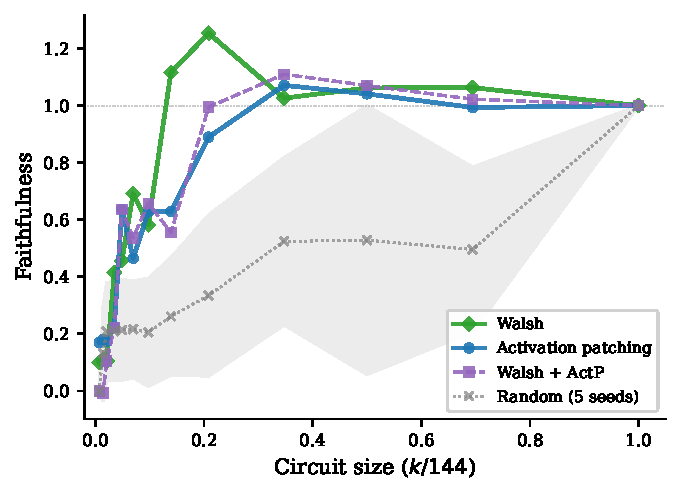
\includegraphics[width=0.7\textwidth]{figures/mib_faithfulness_curves.pdf}
\caption{Faithfulness as a function of circuit size ($k/144$) for
Walsh, activation patching, their rank-sum combination, and random
(mean $\pm$ standard deviation over 5 seeds). Walsh (green diamonds)
leads at small $k$ and reaches $f > 1$ at 20 heads; activation
patching (blue circles) converges more slowly. The gray band shows
the random baseline. All structured methods converge by $k \approx
50$ heads.}
\label{fig:mib-curves}
\end{figure}

